\chapter{Quickstart}
\label{chap:quickstart}
\index{quickstart}

This chapter demonstrates how to get started with \dolfin{}, including
downloading and installing the latest version of \dolfin{}, and solving
Poisson's equation. These topics are discussed in more detail
elsewhere in this manual. In particular, see
Appendix~\ref{app:installation} for detailed installation instructions
and Chapter~\ref{sec:pde} for a detailed discussion of how to solve
partial differential equations with \dolfin{}.

%------------------------------------------------------------------------------
\section{Downloading and installing \dolfin{}}
\index{downloading}
\index{installation}

The latest version of \dolfin{} can be found on the \fenics{} web page:
\begin{code}
  http://www.fenics.org/
\end{code}
The following commands illustrate the installation process, assuming
that you have downloaded release 0.1.0 of \dolfin{}:
\begin{code}
  # tar zxfv dolfin-0.1.0.tar.gz
  # cd dolfin-0.1.0
  # ./configure
  # make
  # make install
\end{code}

Note that you may need to be root on your system to do the last
step. \dolfin{} depends on a number of other packages, including
the linear algebra package PETSc and the form compiler \ffc{}.
(See Appendix~\ref{app:installation} for detailed instructions.)

%------------------------------------------------------------------------------
\section{Solving Poisson's equation with \dolfin{}}
\index{Poisson's equation}

Let's say that we want to solve Poisson's equation on the unit square
$\Omega = (0,1) \times (0,1)$ with homogeneous Dirichlet boundary
conditions on the boundary $\Gamma_0 = \{(x, y) \in \partial \Omega : x = 1\}$,
homogeneous Neumann boundary conditions on the remaining part of the boundary
and right-hand side given by $f = x \sin(y)$,
\begin{eqnarray} \label{eq:poisson,quickstart}
  - \Delta u(x, y) &=& x \sin(y), \quad
  x \in \Omega = (0,1) \times (0,1), \\
  u(x) &=& 0, \quad
  x \in \Gamma_0 = \{(x, y) \in \partial \Omega : x = 1\}, \\
  \partial_n u(x) &=& 0, \quad
  x \in \partial \Omega \setminus \Gamma_0.
\end{eqnarray}

To solve a partial differential equation such as Poisson
with \dolfin{}, it must first be rewritten in \emph{variational form}.
The variational formulation of Poisson's equation reads:
Find $u \in V$ such that
\begin{equation} \label{eq:varform}
  a(v, u) = L(v) \quad \forall v\in \hat{V}, 
\end{equation}
with $(\hat{V}, V)$ a pair of suitable function spaces (the test and
trial spaces). The bilinear form $a : \hat{V} \times V \rightarrow
\R$ is given by
\begin{equation}
  a(v, u) = \int_{\Omega} \nabla u \cdot \nabla v \dx
\end{equation}
and the linear form $L : \hat{V} \rightarrow \R$ is given by
\begin{equation}
  L(v) = \int_{\Omega} f v \dx.
\end{equation}

\subsection{Setting up the variational formulation}
\index{ffc}

The variational formulation (\ref{eq:varform}) must be given to
\dolfin{} as a pair of bilinear and linear forms $(a, L)$ using the
form compiler \ffc{}. This is done by entering the definition of
the forms in a text file with extension \texttt{.form},
e.g. \texttt{Poisson.form}, as follows:
\begin{code}
  element = FiniteElement(``Lagrange'', ``triangle'', 1)

  v = BasisFunction(element)
  u = BasisFunction(element)
  f = Function(element)
  
  a = dot(grad(u), grad(v))*dx
  L = f*v*dx
\end{code}

The example is given for piecewise linear finite elements in two
dimensions, but other choices are available, including arbitrary order
Lagrange elements in two and three dimensions.

To compile the pair of forms $(a, L)$, now call the form compiler on
the command-line as follows:
\begin{code}
  # ffc Poisson.form
\end{code}
This generates the file \texttt{Poisson.h} which implements the forms
in C++ for inclusion in your \dolfin{} program.

\subsection{Writing the solver}

Having now compiled the variational formulation (\ref{eq:varform})
with \ffc{}, it is now easy to implement a solver for Poisson's
equation. We first discuss the implementation line by line and then
present the complete program. The source code for this example is
available in the directory \texttt{src/demo/poisson/} of the \dolfin{}
source tree.

At the beginning of our C++ program, which we write in a text file
named \texttt{main.cpp}, we must first include the header file
\texttt{dolfin.h}, which gives our program access to the \dolfin{}
class library. In addition, we include the header file
\texttt{Poisson.h} generated by the form compiler. Since all classes
of the \dolfin{} class library are defined within the namespace
\texttt{dolfin}, we also specify that we want to work within this
namespace:
\begin{code}
  #include <dolfin.h>
  #include ``Poisson.h''
  
  using namespace dolfin;
\end{code}

Next, we specify the right-hand side $f$ of (\ref{eq:poisson,quickstart}).
This is done by defining a new subclass of \texttt{Function}, which we
here will name \texttt{MyFunction}, and overloading the evaluation
operator to return the value $f(x, y) = x \sin(y)$:
\begin{code}
  class MyFunction : public Function
  \{
    real operator() (const Point& p) const
    \{
      return p.x*sin(p.y);
    \}
  \};
\end{code}

The boundary condition is specified similarly, by overloading the
evaluation operator for a subclass of \texttt{BoundaryCondition}:
\begin{code}
  class MyBC : public BoundaryCondition
  \{
    const BoundaryValue operator() (const Point& p)
    \{
      BoundaryValue value;
      if ( std::abs(p.x - 1.0) < DOLFIN_EPS )
        value = 0.0;
      return value;
    \}
  \};
\end{code}
We only need to specify the boundary condition explicitly on the
Dirichlet boundary. On the remaining part of the boundary, \dolfin{}
assumes homogeneous Neumann boundary conditions by default.

Note that there is currently no easy way to impose non-homogeneous
Neumann boundary conditions or other combinations of boundary
conditions. This will most certainly be added to a future release of
\dolfin{}.

Since we are writing a C++ program, we need to create a \texttt{main}
function.  You are free to organize your program any way you like, but
in this simple example we just write our program inside the
\texttt{main} function:

\begin{code}
  int main()
  \{
    // Write your program here
    return 0;
  \}
\end{code}

The first thing we need to do is to create a mesh. \dolfin{} relies on
external programs for mesh generation, and imports meshes in \dolfin{}
XML format. However, for simple domains like the unit square or unit
cube, \dolfin{} provides a built-in mesh generator. To generate a
uniform mesh of the unit square with mesh size $1/16$ (with a total of
$2\cdot 16^2 = 512$ triangles), we can just type
\begin{code}
  UnitSquare mesh(16, 16);
\end{code}

Next, we initialize the right-hand side, the boundary condition and
the pair of forms that we have previously defined:
\begin{code}
  MyFunction f;
  MyBC bc;
  Poisson::BilinearForm a;
  Poisson::LinearForm L(f);
\end{code}

All that remains is now to assemble the linear system $A x = b$
representing the variational problem (\ref{eq:varform}) and solve for
the vector $x$. To assemble the system, we define a \texttt{Matrix~A},
a \texttt{Vector~b} and call the function \texttt{FEM::assemble()}:
\begin{code}
  Matrix A;
  Vector x, b;
  FEM::assemble(a, L, A, b, mesh, bc);
\end{code}
We may then solve the linear system $A x = b$ for the degrees of
freedom of the solution $u$ using the GMRES method:
\begin{code}
  GMRES solver;
  solver.solve(A, x, b);
\end{code}

Finally, we export the solution to a file for visualization. To do
this, we define a \texttt{Function} which represents a field with
given degrees of freedom in a function space defined by a mesh and a
finite element, which we may obtain from the bilinear form by calling
the member function \texttt{trial()}. Here, we choose to save the
solution in Octave/MATLAB format, which we do by specifying a file
name with extension \texttt{.m}:
\begin{code}
  Function u(x, mesh, a.trial());
  File file(``poisson.m'');
  file << u;
\end{code}

The complete program for Poisson's equation now looks as follows:
\footnotesize
\begin{code}
  #include <dolfin.h>
  #include ``Poisson.h''
  
  using namespace dolfin;

  // Right-hand side
  class MyFunction : public Function
  \{
    real operator() (const Point& p) const
    \{
      return p.x*sin(p.y);
    \}
  \};

  // Boundary condition
  class MyBC : public BoundaryCondition
  \{
    const BoundaryValue operator() (const Point& p)
    \{
      BoundaryValue value;
      if ( std::abs(p.x - 1.0) < DOLFIN_EPS )
        value = 0.0;
      return value;
    \}
  \};

  int main()
  \{
    // Set up problem
    UnitSquare mesh(16, 16);
    MyFunction f;
    MyBC bc;
    Poisson::BilinearForm a;
    Poisson::LinearForm L(f);

    // Assemble linear system
    Matrix A;
    Vector x, b;
    FEM::assemble(a, L, A, b, mesh, bc);

    // Solve the linear system
    GMRES solver;
    solver.solve(A, x, b);
    
    // Save function to file
    Function u(x, mesh, a.trial());
    File file(``poisson.m'');
    file << u;

    return 0;
  \}
\end{code}
\normalsize

\subsection{Compiling the program}

The easiest way to compile the program is to create a
\texttt{Makefile} that tells the standard Unix command \texttt{make}
how to build the program. The following example shows how to write a
\texttt{Makefile} for the above example:
\footnotesize
\begin{code}
  CFLAGS  = `dolfin-config --cflags_dolfin`
  LIBS    = `dolfin-config --libs_dolfin`
  CXX     = `dolfin-config --compiler`

  DEST    = dolfin-poisson
  OBJECTS = main.o

  all: $(DEST)

  install:
  
  clean:
          -rm -f *.o core *.core $(OBJECTS) $(DEST)

  $(DEST): $(OBJECTS)
           $(CXX) -o $@ $(OBJECTS) $(CFLAGS) $(LIBS)

  .cpp.o:
          $(CXX) $(CFLAGS) -c $<
\end{code}
\normalsize

With the \texttt{Makefile} in place, we just need to type
\texttt{make} to compile the program, generating the executable
as the file \texttt{dolfin-poisson}.

\subsection{Running the program}

To run the program, simply type the name of the executable:
\begin{code}
  # ./dolfin-poisson
  Computing mesh connectivity:
  Found 289 nodes
  Found 512 cells
  [...]
  GMRES converged in 21 iterations.
  Saved mesh mesh  [...]
  Saved function u [...]
\end{code}

\subsection{Visualizing the solution}

\dolfin{} relies on external programs for visualization. In this
example we chose to save the solution in Octave/MATLAB format, so we
start Octave (or MATLAB) using the command \texttt{octave}. Then, in
Octave, we import the solution and plot it using the \texttt{pdesurf} command:
\begin{code}
  octave:1> poisson
  octave:2> pdesurf(points, cells, u)
\end{code}
Note that the commands \texttt{pdemesh}, \texttt{pdesurf} and
\texttt{pdeplot} are not included with a standard installation of
Octave, but are available in the subdirectory
\texttt{src/utils/octave/} of the \dolfin{} source tree.

\begin{figure}[htbp]
  \begin{center}
    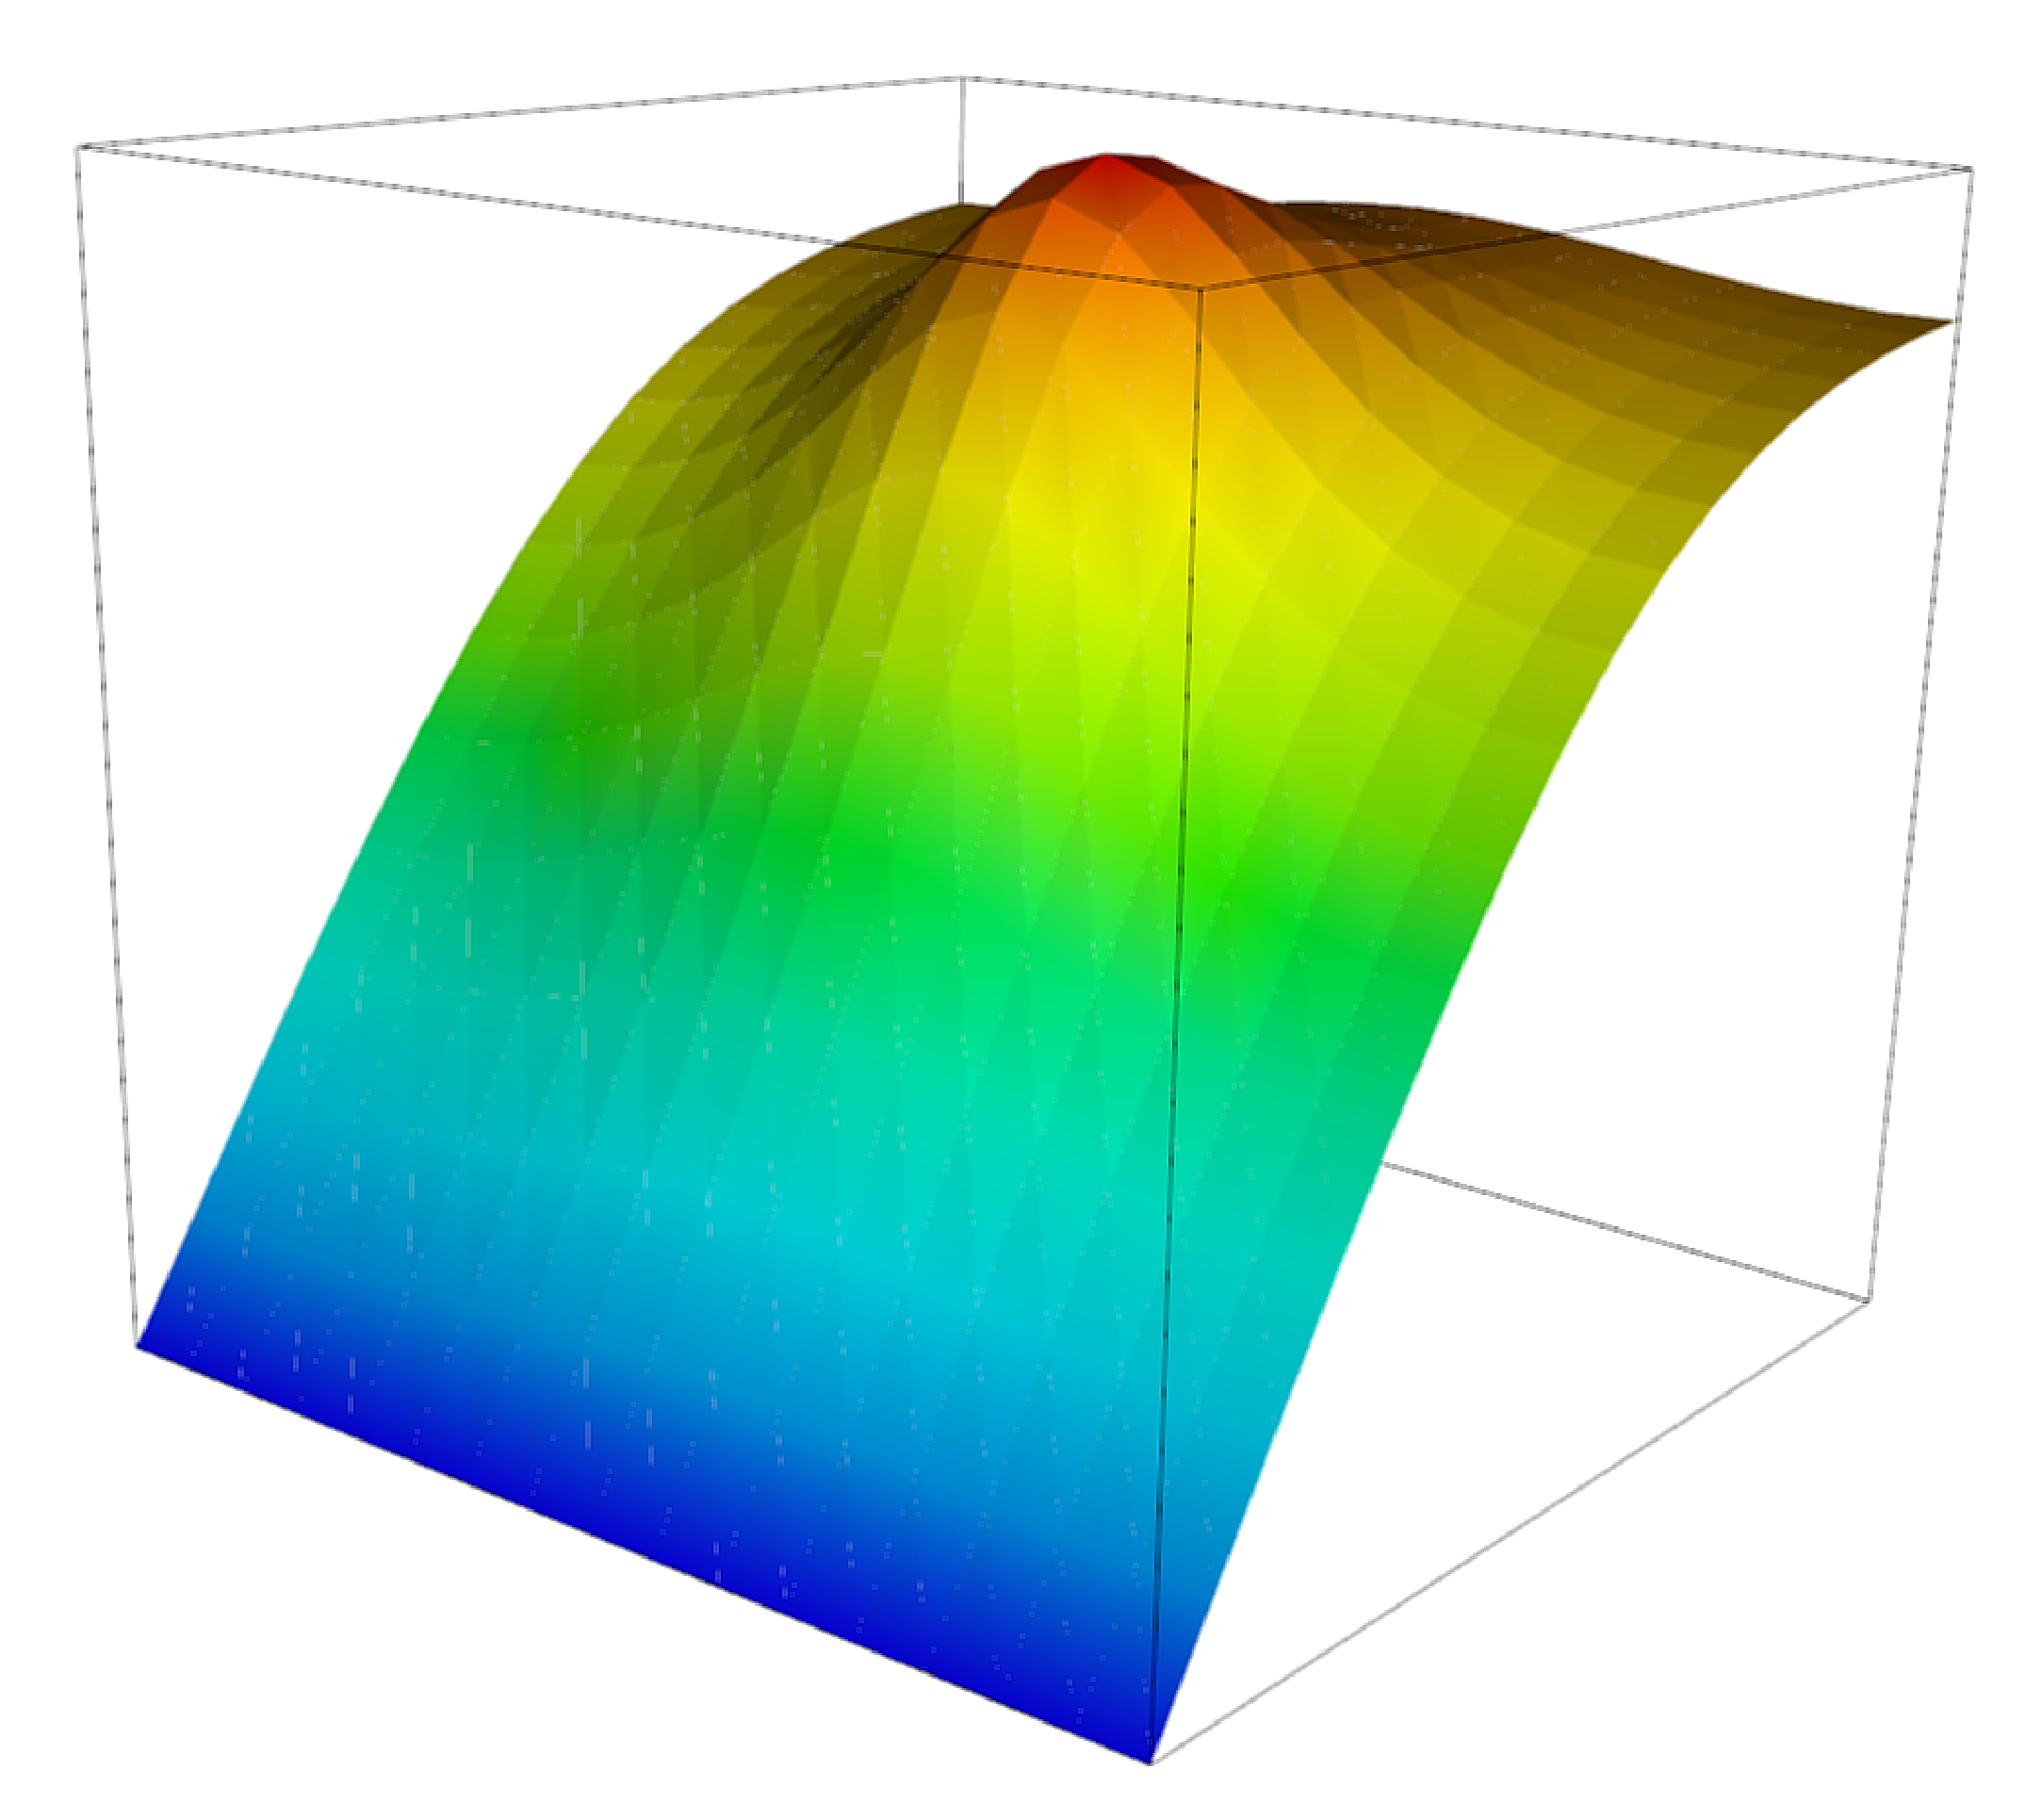
\includegraphics[width=12cm]{eps/poisson.eps}
    \caption{The solution of Poisson's equation (\ref{eq:poisson,quickstart})
      visualized in Octave.}
  \end{center}
\end{figure}
